% !TEX program = xelatex
% !Mode:: "TeX:UTF-8"

% LaTeX template for Chinese essays in psychology
% Author: Yumeng Jiang, Dept. of Psychology, PKU

% Please typeset with xelatex + bibtex + xelatex + xelatex

\documentclass[UTF8,a4paper]{ctexart}

% ==========Preamble==========
\usepackage{apacite}
\usepackage{fancyhdr}
\usepackage{geometry}
\usepackage[font=small,labelfont=bf,labelsep=quad,format=hang,textfont=it]{caption}
\usepackage{booktabs}
\usepackage{graphicx}
\usepackage{float}
\usepackage{xeCJK}

\pagestyle{plain}
\CTEXsetup[format=\Large\bfseries]{section}
\bibliographystyle{apacite}

% ==========Title==========

\title{\bfseries 当代大学生恋爱心理分析} 
\author{李胜锐 \thanks{清华大学软件学院;学号:2017012066;}} 
% Your name in the first blank and your additional information in \thanks{}
\date{\today}
% delete \today if you don't want the date

% ==========Document==========

\begin{document}
% \bibliographystyle{plain}
% \bibliography{ref}{}
% \bibliographystyle{plain}

\maketitle

% ==========Abstract==========

\begin{center}
\parbox{130mm}{\zihao{-5}{\bfseries 摘\quad 要:}
% Abstract here
% An example is as follows
恋爱已经成为了大学生活的一部分。作为年龄和思想观念相近的群体,不同地区大学生对于恋爱的观念都具有高度的一致性。
本文通过综合文献,从大学生恋爱的动机、过程和结局三方面分析当代大学生对于恋爱的普遍心理。
\par
\vspace{1mm}
{\bfseries 关键词:}恋爱\quad 大学生\quad 普遍\quad 心理}
\end{center}

% ==========Body==========

% Example article

\section{前言}
时代在进步,人们的思想观念变化极快。在当代大学生的思想观念中,大学阶段的一段恋爱经历几乎必不可少。由于网络的普及,不同学校、不同背景的大学生可以通过网络充分交流自己的想法和恋爱观念,即使存在恋爱观不同于周围同龄人的学生,也会为了得到爱情迎合主流的思潮。于是,如今时代下,整个中国大学生作为一个群体,恋爱观念有同一化的趋势。这成为了本文将中国大学生作为整体进行研究的基础。

通过在中国知网上大量查询相关论文、研究报告、统计数据,我大致得到了中国大学生恋爱的总体情况,并且对其中的内容进行了总结。在这个基础上,我还结合自己在学校的亲身经济,归纳出了一些普遍存在问题。

\section{文献分析}
\subsection{恋爱动机}
通过查阅文件,我发现在各种报告中,对于大学生恋爱观的刻画非常相似。这足以说明大学生作为一个整体,拥有很高的一致性。综合分析各个文献,在恋爱动机方面,大学生的恋爱有一定的功利性。

文献中指出,当代大学生恋爱观存在的问题,包括盲目性和冲动性。

\textsl{“某些大学生希望寻求美好的大学生 活状态,但又认为校园生活枯燥、没有激情,因此恋爱成为其摆脱寂寞的 最佳方式。大学生最初积累专业知识、生活技能以及社会经验的时期就是 大学时光,个别大学生将增加作为生活一部分的恋爱经验作为校园恋爱的 直接原因。”}\citeA{:jxm}

\textit{
“部分大学生将恋爱当做一种时尚与攀 比,为了恋爱而去恋爱,而且大学校园中这种跟风恋爱现象有蔓延的趋势。另外还有一部分大学生将物质条件、外貌长相等放在选择恋爱对象的第一位,以期通过恋爱行为满足虚荣心。”}\citeA{:jxm}

所谓“动机不纯”可以说是形容这种恋爱动机的最好的方式。

而另一篇文献中也提到了这一点,作者指出,大学生恋爱有很多不成熟的心理,其中包括从重心理、虚荣心理以及功利性心理。\citeA{:lxj}很多大学生并不是出于真正的爱慕对方,想要和对方一起走下去的目的进行恋爱。相反,在很多情况下,大学生谈恋爱是为了弥补空虚、孤独的从众心理,有的人甚至认为拥有男朋友或者女朋友是实力的象征。

在这种条件下,很多爱情都走向了悲剧。这也是现在大学生情侣之间分手率非常高的原因之一。

当然以上情况只是大学生恋爱动机的一部分,而总体上的情况并没有这么糟糕。一些可靠的统计数据表明,大多数大学生对爱情的态度处于一种较为纯洁的层次,他们确实渴望美好的爱情,而他们的恋爱动机是“互相关心,互相帮助,共同进步。”\citeA{:wyl}这说明,这些大学生在大学中寻找异性伴侣,更多的是为了彼此之间能够在学习生活中互相陪伴。这显然是一种非常积极阳光的恋爱观,可以认为是最能使情侣在大学中收获更纯真、更美好爱情的恋爱观。

而提到两个人是处于什么原因走到一起,大多数调查研究表明\citeA{:wyl},很大程度上是由于两人“一见钟情”。这体现了心理学上的首因效应。由于大学生活有很多机会接触到异性,所以大学生择偶的选择范围相对比较大,有更多的选择。但是,很多接触仅仅只是建立在表面,同学之间并没有机会进行深入交流。所以,决定一个人吸引力的内在因素很难体现出来,更多的吸引体现在外表上。在这种基础上,再加上首因效应的影响,所以第一印象对于大学生建立吸引力非常关键。

\subsection{恋爱过程}
当代大学生具体的恋爱的方式也是一个非常有趣的话题。对于这个问题,我从文献中找到了很多方面的描述,下面就从各个方面逐一阐释。

\subsubsection{性观念}
如果可以用一句话概括当代大学生对于性的看法,那就是:新一代比老一代更加开放,男生比女生更加开放。

\textit{
“大学生发生性关系现状 对于大学生发生性
关系的人数调查结果显示,17 名男生(27.93 \%)和 87 名女生(12.97 \%)表示自己已经发生过性关系。”}\citeA{:ylp}

\textit{
“关于大学生发生性 行为的观点,男生选择“完全赞同,这很正常”“无特 别意见,可以接受”“最好不要,大学生要矜持自重” “完全反对,绝对不可以”的分别为 125 人(20.06 \%)、 288 人(46.23 \%)、192 人(30.82 \%)、18 人(2.89 \%), 女生分别为 94人(14.01 \%)、311人(46.35 \%)、 247 人(36.81 \%)、19 人(2.83 \%),差异有统计学意 义(χ2 = 10.42,P < 0.05)。问及大学生发生性行为的 原因,选择“显示爱情忠贞”“追求快乐”“生理需求” “避免孤独”的男生分别为 84 人(13.48 \%)、152 人 (24.4 \%)、352 人(56.5 \%)、35 人(5.62 \%),女生分 别为 282人(42.03 \%)、119人(17.73 \%)、227人 (33.83 \%)、43 人(6.41 \%),差异有统计学意义(χ2 = 137.35,P < 0.01)。”}\citeA{:ylp}

从统计数据中可以看出,超过四分之一的男生和超过八分之一的女生已经发生过性关系。可见,在大学发生性关系已经是很普遍的现象,相对更加开放的男生发生性关系的比例更高。

而另一份文献中,更加深入地研究了大学生对于性观念的态度。以下是截取自文献中的研究统计数据\citeA{:lhs}:

\begin{figure}[ht]
    \centering
    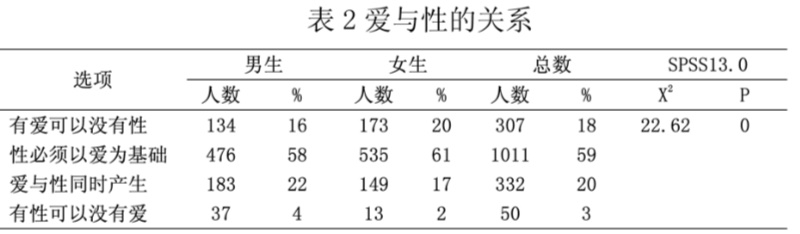
\includegraphics[scale=0.4]{2.jpg}
    % \caption{this is a figure demo}
    % \label{fig:label}
    \end{figure}
    
\begin{figure}[ht]
    \centering
    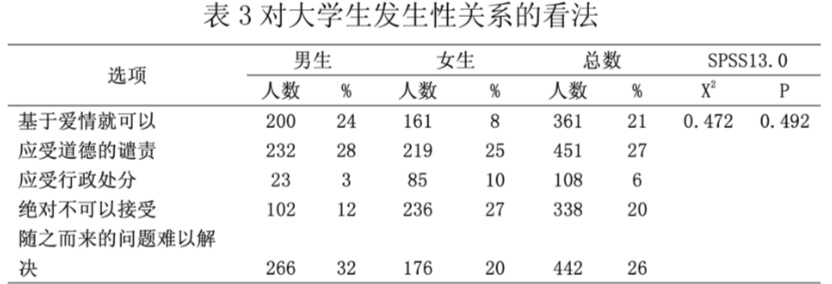
\includegraphics[scale=0.4]{3.jpg}
    % \caption{this is a figure demo}
    % \label{fig:label}
    \end{figure}

\begin{figure}[ht]
    \centering
    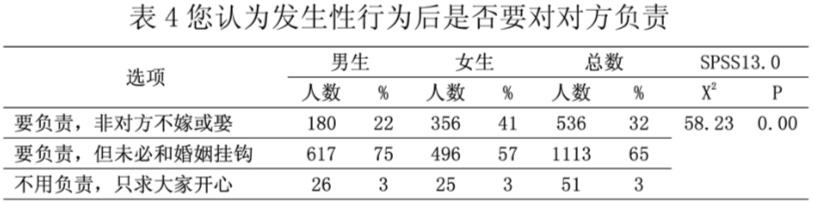
\includegraphics[scale=0.4]{4.jpg}
    % \caption{this is a figure demo}
    % \label{fig:label}
    \end{figure}

\begin{figure}[ht]
    \centering
    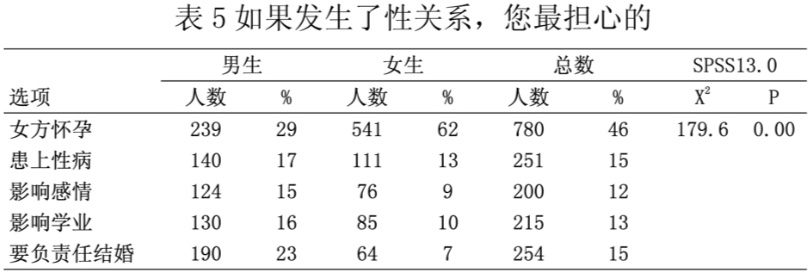
\includegraphics[scale=0.4]{5.jpg}
    % \caption{this is a figure demo}
    % \label{fig:label}
    \end{figure}

\begin{figure}[ht]
    \centering
    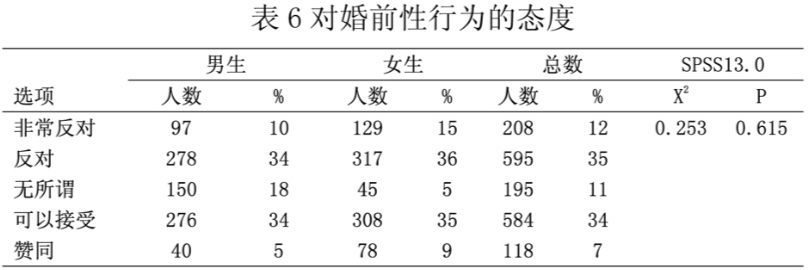
\includegraphics[scale=0.4]{6.jpg}
    % \caption{this is a figure demo}
    % \label{fig:label}
    \end{figure}

\begin{figure}[h!]
    \centering
    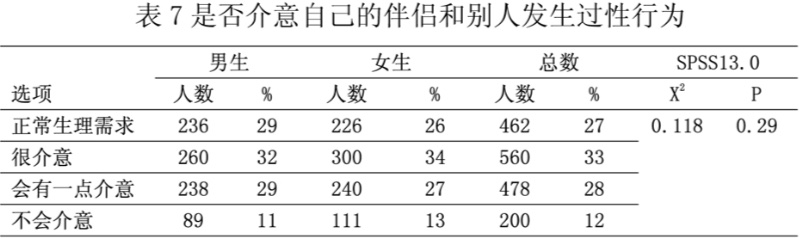
\includegraphics[scale=0.4]{7.jpg}
    % \caption{this is a figure demo}
    % \label{fig:label}
    \end{figure}

从表2统计数据中可以发现,绝大多数大学生把性当作一件爱情中不可或缺的内容,这是认为是一种正确的观念。而在大学生是否应该发生性关系上,这篇文献表3的结果和之前的结果基本一致,有一定比例的学生可以接受大学期间的性行为,女生接受程度更低;表4指明绝大多数大学生会在发生性关系后对对方负责;表5表明发生性关系后,又一个很有趣的现象是,女生主要害怕自己怀孕,而男生不仅害怕对方怀孕还害怕要为对方负责;表6表明对于婚前性行为,男生女生基本上都是一般接受一般反对,性别差异不明显;表7表明,大多数人还是会介意对方有过性行为,但这种介意已经没有达到无法接受的程度了,这表明当今社会的对婚前性行为的包容程度已经比较比较高了。

\subsubsection{爱情的单纯性}
学生时代的恋爱最有明显的特征就是单纯性,大学生在恋爱过程中很少关注对方的家庭和物质财富。

\textit{
“单纯而美好的大学生大部分时间都生活在校园里, 很少有机会在社会大环境中历练,恋爱双方基本不会考虑家庭和物质财富 等因素,他们认为只要彼此有感觉就有在一起的基础。另外闪恋、闪婚等 词语的出现,也能体现出在恋爱过程中当代大学生所追求的速度以及强烈 的恋爱需求。”}\citeA{:jxm}

不过,单纯性也有其不好的一面。很多大学生忽略了爱情三角理论中承诺这一方面。在一些极端情况下,他们把恋爱当作一种情感体验、当作一种游戏 和消遣文化,当作派遣寂寞、赶走孤单的工具和手段,寻求刺 激,及时行乐,满足所谓的感觉或精神享受,其实质是只强调爱的权利,否认爱的责任和义务,其结果只能是既伤害对方, 又伤及自己。\citeA{:yyq}这也是导致毕业即分手这一现象越来越普遍的原因。

从我个人的经历来说,现在周围流传着一种说法,认为大学期间的恋爱才是最纯洁的,它少了很多世俗的气息,以后走出校园,很难遇到合适的人。这种说法印证了文献中谈及的单纯性这一特点。所以,大学期间的爱情的单纯性是非常有依据的。

\subsubsection{爱情与学业}
调查表明,虽然超过 90\%的大学生认为自己必须正确看待学业与爱情的关系,学习是学生的天职,所以大学生必须以学习为主,学
习第一,爱情第二,或者学业与爱情双丰收,既希望学业有成,又渴望爱情幸福。但是,在客观实际上,即使有这样的想法,真正能够处理好学业与爱情关系的只有占极少数学生。更多的学生一旦堕入情网就难以自拔,情不自禁,想入非非,沉迷于卿卿我我的甜言蜜语、男欢女爱中。\citeA{:yyq}

而这所谓90\%的学生很多只是有这种观念,实际上,由于爱情是一种非常感性的存在,大学生又处于青春懵懂之时,对于爱情完全没有抵抗力。因此,很多时候,他们自然而然置其他于不顾,最后也在一定程度上耽误了自己的发展。

不过,依然有很多人认为,大学爱情在很大程度上帮助了大学生学习。从通常的理解来看,两个人如果都积极向上热爱学习,他们更多时间是在督促对方变得更优秀。如果能够利用爱情的力量帮助对方成长,那爱情对于双方来说都是一件好事。

\textit{
“大学生希望能够有更多的时间和 对方了解并磨合与沟通, 在处理恋爱和学业的冲突时 大部分人选择了后者, 说明大多数人对于恋爱还是有 正确认识的,作为学生应该把学业放在第一位。”}\citeA{:zxt}

\subsection{恋爱结局}

\subsubsection{毕业}

众所周知,大学期间的爱情,正所谓有情人多,终成眷属者少。能走到最后的人,是极少的一部分。大学情侣往往难以逃脱最终分手的命运。

处于恋爱中的双方作为成年人不仅面临学业的问 题,还面临着毕业后距离上分开如是否出国深造、是否 异地、是否分手等各种现实问题。 个性特点比较鲜明的 新时代大学生面对感情问题也是比较自我。其中当爱情、考研或出国发生冲突如何选择时,57.81\%的学生选 择坚持自己的选择,只有 14.06\%的学生会选择追随对方。 同时,在问题是否为双方未来发展进行沟通以及做相应努力方面,大家普遍表示有所沟通,但是努力不够。\citeA{:zxt}

从这一点可以看出,毕业之后的分手,并不完全是出于情侣双方的无奈。实际上可以说,双方早就预见到了会有这种情况的发生。当自己的人生规划和伴侣之间出现非常严重的冲突时,两人往往不会选择尊重爱情,而是选择自己的前途。

\subsubsection{失恋}
大学生与成年人相比,由于心智不完全成熟,具有较弱的恋爱抗压性。一项数据表明,大学生自杀的人数中,因为感情选择自杀的比例,达到了三分之一。

当然,除了自杀这种极端情形,大学生在失恋之后采取的更多的往往是报复、转移注意力和自我提升。

\textit{
“在 受 调 查 的 女 生 中 ,有 95 人 选 择 “C .分 析 原 因 ,自 我 完 美 ”,占 44.19\% ;有 58 人 选 择 了 “F.痛 苦 ,但 可 以 转移注意力,靠时间恢复”,说明大部分的大学生对于 失恋是比较理性的,这一部分人可以从失败中吸取教 训,从而完善自己,并且可以从失恋中走出来,自我恢 复 。 其 中 ,有 19 人 选 择 了 “B.报 复 对 方 ”,这 一 比 例 达 到 了 8 .8 4 \% 。 面 对 全 国 大 学 生 的 数 量 , 这 一 比 例 不 容 忽 视 ,说 明 大 约 有 8 .84 \% 的 女 生 在 恋 爱 中 不 容 易 走 出 来,并且产生了报复心理,这一心理对于大学生的心理 健康会有很大的影响。
在 受 调 查 的 男 生 中 ,有 204 人 选 择 “C .分 析 原 因 , 自我完美”,占42.68\%,这一比例与受调查的女生相 似 ;有 112 人 选 择 “F .痛 苦 ,但 可 以 转 移 注 意 力 ,靠 时 间 恢 复 ” , 占 2 3 .4 3 \% , 这 一 比 例 也 与 女 生 相 似 。 说 明 大 部 分的学生都可以靠自己走出失恋的阴影,并且从中吸 取 教 训 。35 人 选 择 “G.其 他 ”,29 人 选 择 “B.报复对方””}\citeA{:zxt}

失恋不可怕,可怕的是失恋之后失去志向、失去品德。从调查结果来看,大部分男生女生对待失恋的态度比较相似。大多数大学生都可以做到从失恋中吸取教训,提升自己,从而很快恢复。选择报复甚至自杀的还是极少数。所以,可以说失恋并不可怕,能从一段失败的感情经历中学到东西,反倒是可贵的一件事。

总而言之,勇敢地去追寻爱情吧!

\section{相关理论}
大学生恋爱有很多地方可以从心理学的角度去研究的。

\subsection{从爱情风格理论分析大学生恋爱的风格偏向}
文献中很多地方都谈及到了大学生恋爱的特点,而往往可以通过这些特点划分爱情的风格。由于大学生群体恋爱有一致性的趋势,所以大学生的爱情风格也有一定的一致性。

大学生恋爱各种风格都会存在,但只有某些特定的风格,往往可以最终保持爱情的长久。

由于大学生的社交圈重合度比较大,对待爱情会更加谨慎,也更会考虑长远。否则,一旦日后关系破裂,情侣双方可能甚至同在一个院系甚至一个班,见面会非常尴尬。即使不在同一个院系,由于双方同时认识的人非常多,爱情的破裂对于人际关系也是一种考验。因此,这也可以视为一种得天独厚的“优势”。它杜绝了很多短期的恋爱关系。通过以上分析,可以看出,游戏之爱存在的比例会比现实中低很多。即使双方都抱着“玩一玩”的想法,也很难摆脱人际关系的束缚,真正地只是“玩一玩”。

同时,由于大学生恋爱的单纯性,大学生群体不会倾向于考虑现实的因素,不会为了以后的生计,不会为了柴米油盐的琐事担忧。因此,现实之爱的比例会非常低,甚至很难在校园中存在。

另外,大学生的恋爱对象大多是有共同话题,志趣相投的人。由于校园内可以接触到形形色色的同龄人,选择的范围非常广,比较的范围也非常多,所以很难存在双方差异很大却恋爱的情况。基于这样的事实,双方实力会非常对等,所以自我牺牲的奉献之爱在大学中不常见。

所以,个人认为,大学校园中最为常见的恋爱形式是浪漫之爱、占有之爱和友谊之爱。六种爱情风格的分布比例和社会中的分布比例有明显的不同。

\subsection{从爱情三元素分析“承诺”缺失的影响}
“承诺”在校园爱情中的缺失几乎已经成为了一个普遍现象。在校大学生升学之后的去向没有确定,正如前文提及,绝大多数大学生在面临去向选择时,会优先考虑个人的利益。当然这也是如今社会风气所致,事实上,社会也并不提倡学生为了爱情改变自己的人生追求。

所以,承诺的缺乏,导致大学生爱情更多的是靠亲密和浪漫维系。这也是现实之爱几乎不存在的重要原因。

不过,虽然很少有长期的承诺,短期的承诺对于大学生爱情的维系仍然必不可少。大学生稳定的爱情大多包含有短期的承诺,而不是长期的承诺。可见,短期承诺实际上已经对爱情的维系起了很大的作用。

长期承诺的缺失,导致大多数大学生的想法并不是于另一半厮守终身。他们更多得是想找到一个可以在大学陪伴自己的人,对于这份感情并没有走到最后的信心。

\subsection{从文化的影响分析大学生爱情的发展趋势}

中国的婚姻文化随时代而变化。
从最开始的父母之命,媒妁之言变成了自由恋爱;从最开始的妻妾成群变成了一夫一妻特定的婚姻习俗。结婚的年龄也逐年提高。同时,中国的婚姻文化在很大程度上也收到了外国尤其是西方的影响。婚前适婚以及同居的现象越来越常见。

这些社会现象显著影响着大学生的恋爱观。大学生变得更加开放。

所以,随着社会进一步的变得开放,大学生的恋爱观也会随着社会的变化而变化。相信以后,大学生的恋爱方式也会变得更加开放,变得和如今很多西方国家相似。这也会带来一些社会上的问题,比如性观念的过于开放,可能导致不安全的性行为增多,大学生的健康受到威胁等。总之,我们要对这一变化有预见性。




% ==========References==========
 \renewcommand\refname{参考文献}
% enter your .bib file name in the parentheses in the following line.
\bibliography{ref}



\end{document}

